\documentclass[a4paper, 11pt]{article}
\usepackage{comment} % enables the use of multi-line comments (\ifx \fi)
\usepackage{lipsum} %This package just generates Lorem Ipsum filler text.
\usepackage{fullpage} % changes the margin
\usepackage{graphicx}
\usepackage{float}

\begin{document}
%Header-Make sure you update this information!!!!
\noindent
\large\textbf{C++ Assignment 2} \hfill \textbf{Jiecheng Song} \\
\normalsize AMS 595 \hfill SBID:111783762 \\
Prof. Barbara Chapman \hfill Lab Date: 12/03/2017 \\
TA: Xiaoyu Li \hfill Due Date: 12/03/2017

\section*{Introduction to the code
}
When we execute the code, it will ask us to input the N, which will be the max times of the iterations. After input, what the number you input will show and the difference (RMS) of the last two iterations will show, as well as the execution time. If what you input is not positive or not a number, the default level of accuracy and the difference (RMS) of the last two iterations and the execution time will be shown.\\
Since I found if we set N as an integer, if we input string or other type variables into N, N will be recognized as 0, so we use if N is over 0 as a condition to decide to use max times iterations or default level of accuracy.

\section*{Performances of Jacobi Method}
\begin{figure}[H]
\centering
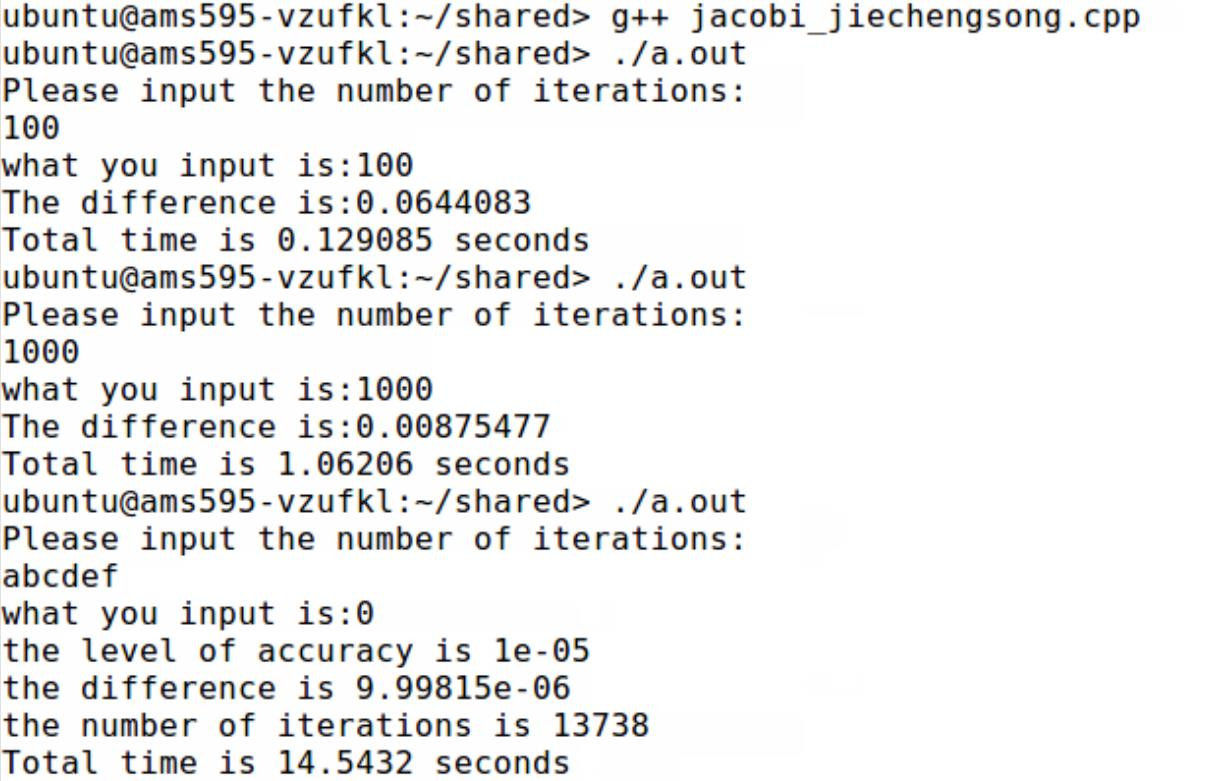
\includegraphics[width=\textwidth]{jacobi1.jpg}
\caption{examples for function test}\label{fig:digit}
\end{figure}
\begin{figure}[H]
\centering
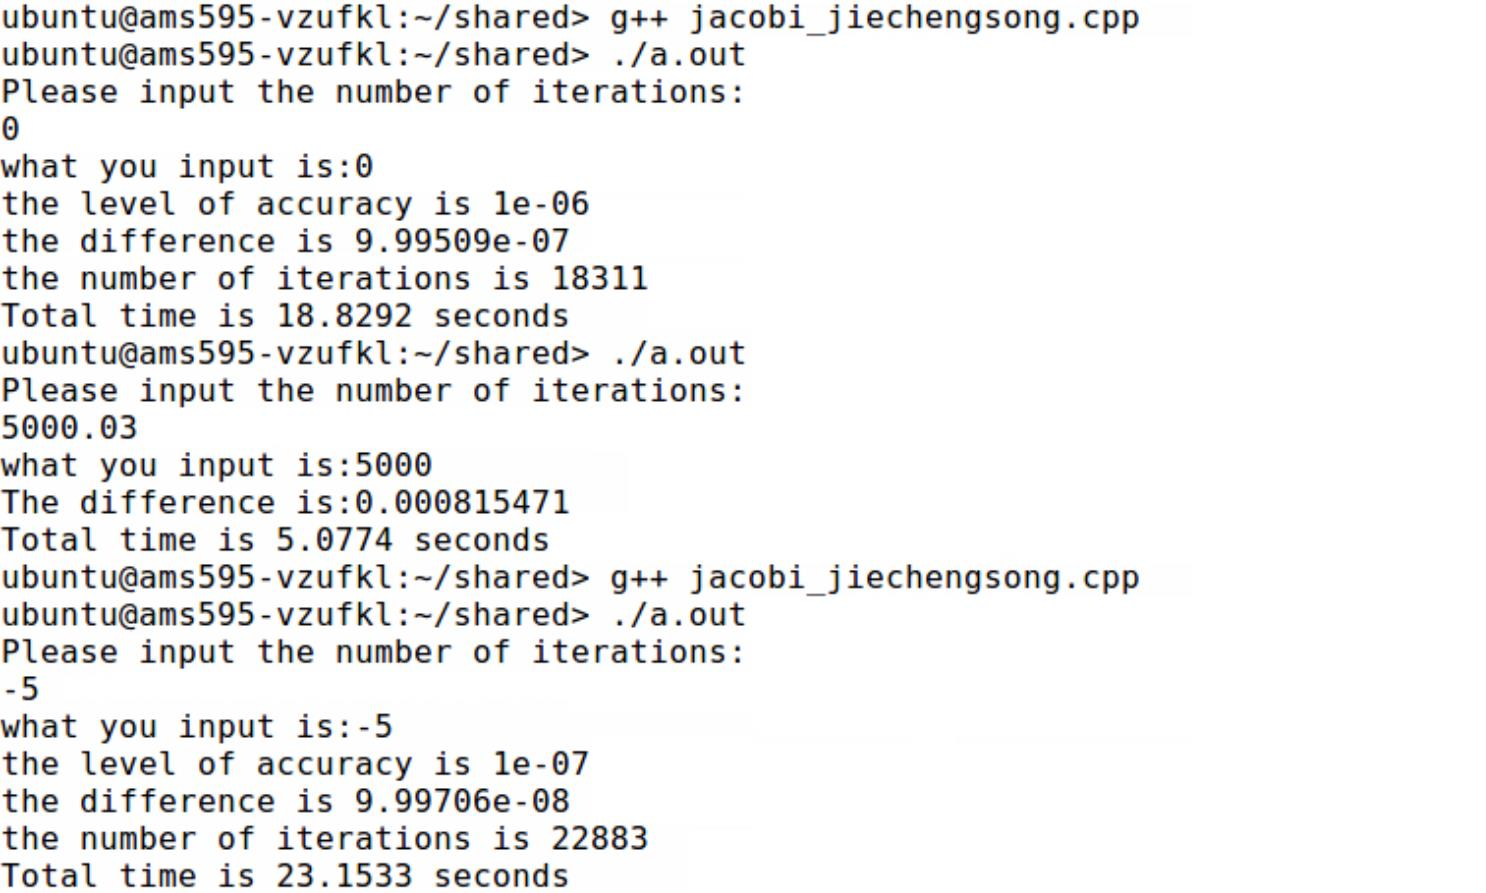
\includegraphics[width=\textwidth]{jacobi2.jpg}
\caption{examples for function test}\label{fig:digit}
\end{figure}
\section*{Performances of Gauss-Seidel Method}
\begin{figure}[H]
\centering
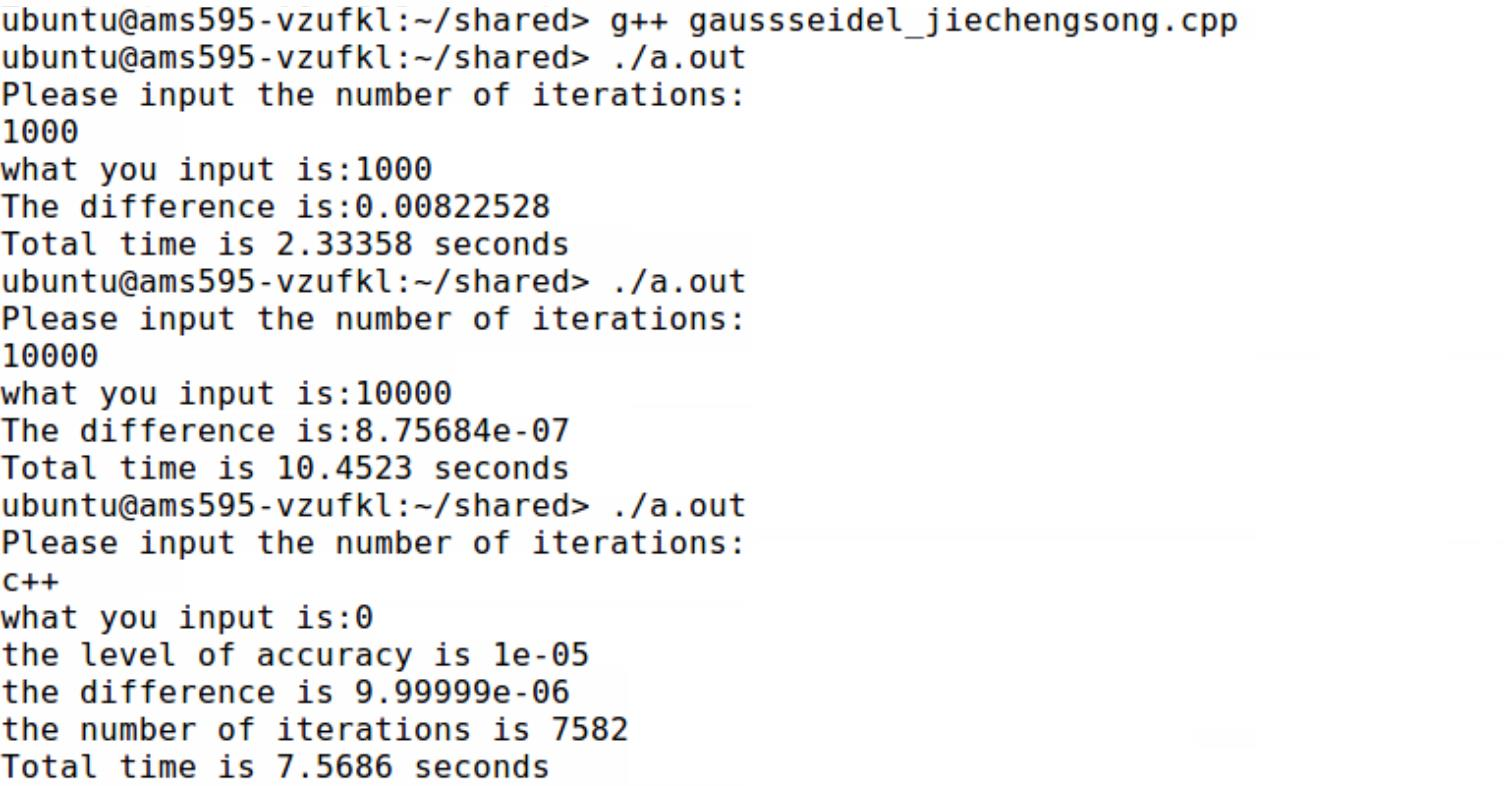
\includegraphics[width=\textwidth]{gauss1.jpg}
\caption{examples for function test}\label{fig:digit}
\end{figure}
\begin{figure}[H]
\centering
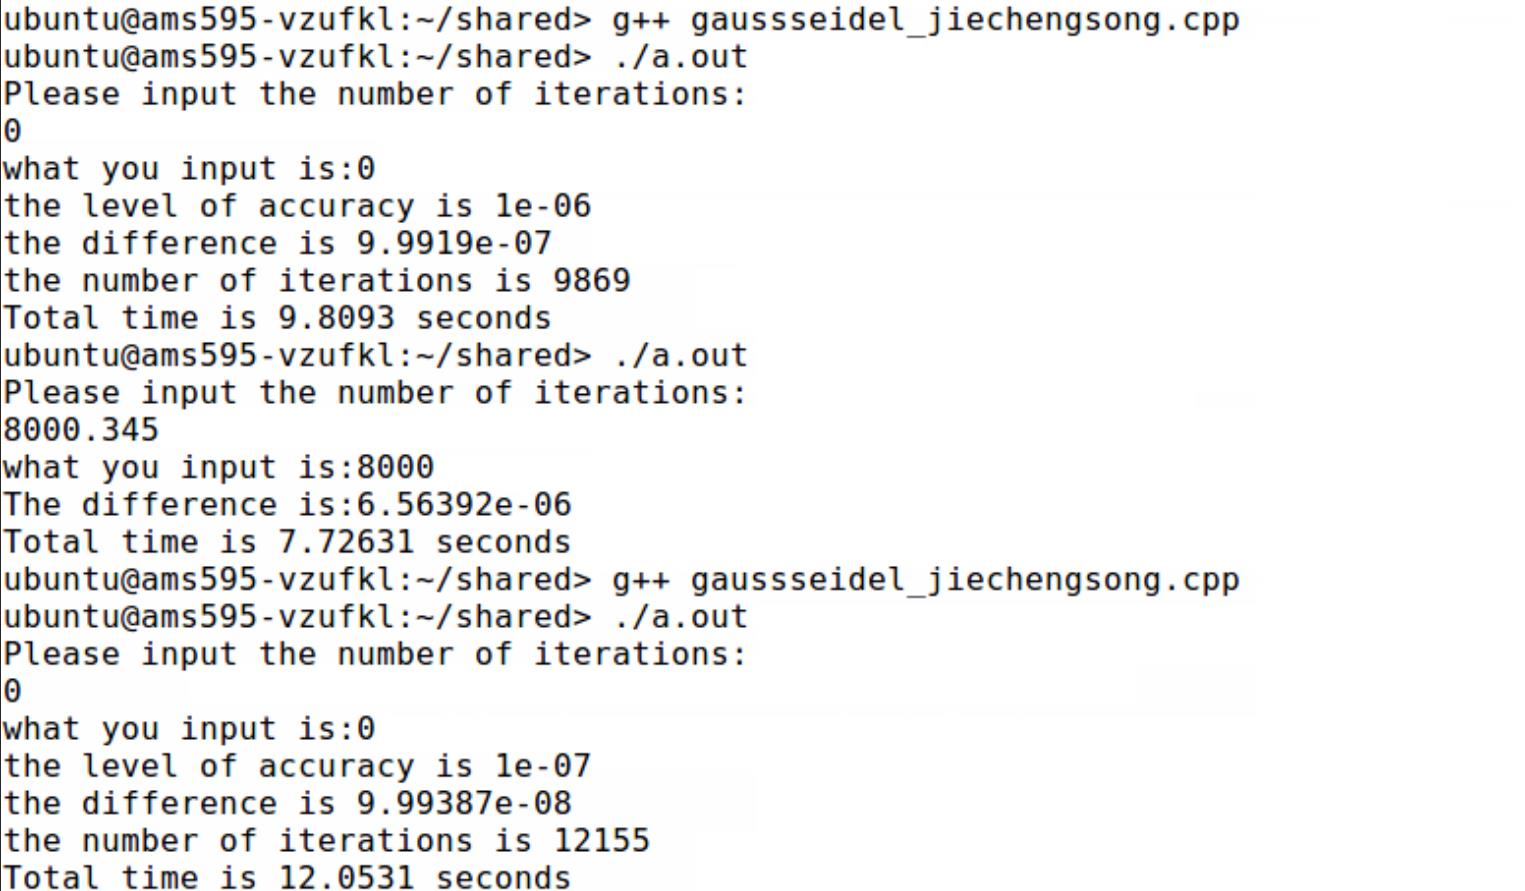
\includegraphics[width=\textwidth]{gauss2.jpg}
\caption{examples for function test}\label{fig:digit}
\end{figure}
\section*{Conclusion}
We can find that using Gauss-Seidel Method will cost similar time with Jacobi Method with the same max iteration times. But with the same level of accuracy, it will also cost less time and times of iterations.
\end{document}
